\documentclass[12pt,a4paper]{article}
\usepackage[utf8]{inputenc}
\usepackage[T1]{fontenc}
\usepackage[croatian]{babel}
\usepackage{geometry}
\usepackage{graphicx}
\usepackage{setspace}
\usepackage{titlesec}
\usepackage{fancyhdr}
\usepackage{caption}
\usepackage{longtable}
\usepackage{array}
\usepackage{tabularx}
\usepackage{amsmath}
\usepackage{amssymb}
\usepackage{mathptmx}       % Times New Roman font
\usepackage{chngcntr}       % Za numeriranje po poglavljima
\usepackage[hidelinks]{hyperref}       % Za URL linkove bez ružnih okvira

% Postavke margina
\geometry{left=2.5cm,right=2.5cm,top=2.5cm,bottom=2.5cm}

% Prored 1.5
\onehalfspacing

% ---- STILOVI NASLOVA ----
\titleformat{\section}
  {\normalfont\large\bfseries\uppercase}{\thesection.}{0.5em}{}
\titleformat{\subsection}
  {\normalfont\normalsize\bfseries}{\thesubsection.}{0.5em}{}
\titleformat{\subsubsection}
  {\normalfont\normalsize\bfseries\itshape}{\thesubsubsection.}{0.5em}{}
\titleformat{\paragraph}[hang]
  {\normalfont\normalsize\itshape}{\theparagraph.}{0.5em}{}
\titlespacing*{\paragraph}{0pt}{3.25ex plus 1ex minus .2ex}{0.5em}

% Svaki \section počinje na novoj stranici
\newcommand{\sectionbreak}{\clearpage}

% ---- NUMERIRANJE SLIKA, TABLICA I JEDNADŽBI PO POGLAVLJIMA ----
\counterwithin{figure}{section}
\counterwithin{table}{section}
\counterwithin{equation}{section}

% Dubina numeriranja (do 4 razine)
\setcounter{secnumdepth}{4}
\setcounter{tocdepth}{4}

% ---- NAZIVI AUTOMATSKIH POPISA ----
\addto\captionscroatian{%
  \renewcommand{\contentsname}{SADRŽAJ}%
  \renewcommand{\listfigurename}{POPIS SLIKA}%
  \renewcommand{\listtablename}{POPIS TABLICA}%
  \renewcommand{\refname}{LITERATURA}%
}

% ---- POTPISI SLIKA I TABLICA ----
\captionsetup[figure]{font={small,bf},labelsep=period}
\captionsetup[table]{font={small,bf},labelsep=period,position=above}

% ---- ZAGLAVLJE I PODNOŽJE ----
\pagestyle{fancy}
\fancyhf{}
\fancyhead[L]{\small\textit{Krešimir Hartl}}
\fancyhead[R]{\small\textit{Zadatak pick-and-place voća}}
\fancyfoot[L]{\small\textit{Fakultet strojarstva i brodogradnje}}
\fancyfoot[R]{\small\textit{\thepage}}
\renewcommand{\headrulewidth}{0.4pt}
\renewcommand{\footrulewidth}{0.4pt}

\begin{document}

% =====================================================================
% NASLOVNICA
% =====================================================================
\begin{titlepage}
    \thispagestyle{empty}
    \centering
    {\fontsize{16pt}{19pt}\selectfont SVEUČILIŠTE U ZAGREBU\\}
    {\fontsize{16pt}{19pt}\selectfont FAKULTET STROJARSTVA I BRODOGRADNJE\\}
    \vfill
    {\fontsize{28pt}{34pt}\selectfont\bfseries HUMANOIDNI ROBOTI I BIOMIMETIČKI SUSTAVI\\}
    \vspace{0.5cm}
    {\fontsize{28pt}{34pt}\selectfont\bfseries ZADATAK PICK-AND-PLACE VOĆA\\}
    \vfill
    \noindent
    \begin{minipage}[t]{0.48\textwidth}
        \raggedright
        {\fontsize{14pt}{17pt}\selectfont \ \\}
        {\fontsize{14pt}{17pt}\selectfont \ \\}
    \end{minipage}
    \hfill
    \begin{minipage}[t]{0.48\textwidth}
        \raggedleft
        {\fontsize{14pt}{17pt}\selectfont\bfseries Krešimir Hartl\\}
    \end{minipage}
    \vspace{1cm}
    \begin{center}
        {\fontsize{14pt}{17pt}\selectfont Zagreb, 2026.}
    \end{center}
\end{titlepage}

% =====================================================================
% SADRŽAJ I POPISI (rimske stranice)
% =====================================================================
\pagenumbering{Roman}

\tableofcontents
\newpage
\listoffigures
\newpage

% =====================================================================
% SADRŽAJ RADA (arapske stranice)
% =====================================================================
\pagenumbering{arabic}

\section{ARHITEKTURA SUSTAVA}
Arhitektura programskog rješenja izvedena je po načelima objektno-orijentiranog programiranja s jasnim razdvajanjem dužnosti kroz \textit{adapter} uzorke dizajna. Sustav se sastoji od sljedećih ključnih modula:
\begin{itemize}
    \item \textbf{VisionAdapter}: Zadužen za sučeljavanje s RGB-D kamerom (ili offline spremljenim podacima), izvršavanje YOLO detekcije, izradu Point Cloudova i upravljanje modelima prepoznavanja voća.
    \item \textbf{PointCloudProcessor}: Domenski modul unutar vizualnog adaptera koji se bavi isključivo prostornom geometrijom (filtriranje $Z$-osi, uklanjanje šuma, DBSCAN klasteriranje, te ICP registracija za spajanje više pogleda).
    \item \textbf{RobotAdapter}: Služi kao komunikacijski most prema UR robotu putem RTDE sučelja. Obavlja micanje robota (J i L gibanja), primjenu \textit{task-space} putanja i slanje digitalnih signala za pneumatsku hvataljku (DO 4 za otvaranje, DO 5 za zatvaranje, 0.5s trajanje pulsa).
    \item \textbf{PlanningUseCase}: Modul u kojem se implementira logika rješavanja problema. Izračunava kvintičku interpolaciju (polinomi petog stupnja) između zadanih pozicija (Home, Approach, Pick, Approach Place, Place) vodeći računa o maksimalnim brzinama i ubrzanjima.
    \item \textbf{PipelineOrchestrator}: Centralni orkestrator koji povezuje gornje module te osigurava pravilan redoslijed izvršavanja, upravlja spremanjem međurezultata i prelaskom iz stanja \textit{Perception} u \textit{Planning} i \textit{Execution}.
\end{itemize}

\section{KALIBRACIJA SUSTAVA}
Hand-Eye kalibracija i dobivanje unutarnjih parametara kamere (intrinzična kalibracija) odrađeni su sljedećim postupkom:
\begin{itemize}
    \item \textbf{Kalibracijski uzorak}: Korišten je ChArUco plakat dimenzija $5 \times 7$. Parametri u kodu sustava za detekciju točaka postavljeni su na \texttt{board = cv2.aruco.CharucoBoard((5, 7), 0.0291, 0.0146, aruco\_dict)}, što definira da je duljina polja $29.1$ mm, a duljina markera $14.6$ mm.
    \item \textbf{Prikupljanje podataka}: Sustav je obradio 26 RGB slika iz različitih statičnih poza robota kako bi se dobila visoka varijansa kuteva i translacija u radnom prostoru.
    \item \textbf{Metoda rješavanja}: Homogena matrica transformacije između baze kamere i baze robota izračunata je korištenjem robusne \texttt{cv2.calibrateHandEye} metode.
\end{itemize}

Konačna kalibracijska matrica $T_{\text{cam\_from\_tcp}}$ (kamera u odnosu na TCP) koja se koristi u sustavu dana je ispod:
\begin{equation}
T_{\text{cam\_from\_tcp}} = \begin{bmatrix}
-0.38711 & -0.84345 & -0.37245 & 0.12537 \\
 0.92193 & -0.34825 & -0.16955 & 0.02687 \\
 0.01330 & -0.40902 &  0.91242 & -0.11331 \\
 0.00000 &  0.00000 &  0.00000 & 1.00000
\end{bmatrix}
\end{equation}

\section{OBRADA POINT CLOUD PODATAKA}
Za svaki od tri pogleda (s različitih stajališta robota), generiran je oblak točaka korištenjem dubinske slike, RGB slike te kamernih intrinzičnih parametara (fokalne duljine i optički centar). Nakon generiranja sirovog Point Clouda, odrađeni su sljedeći koraci:
\begin{enumerate}
    \item \textbf{Filtriranje po Z osi}: Odbačene su točke izvan radnog područja stola (kako bi se eliminirali pod, strop i zidovi).
    \item \textbf{Statističko filtriranje šuma}: Korišten je algoritam za odbacivanje točaka koje su prosječno previše udaljene od svojih $k=20$ najbližih susjeda s devijacijom $std\_ratio=2.0$. Time su smanjene refleksije i šum s rubova objekata.
    \item \textbf{Segmentacija}: Koristeći 2D maske dobivene preko YOLO modela (s pragom $conf=0.75$), 3D točke unutar maske su izdvojene, a zatim provučene kroz 3D DBSCAN ($eps=0.03$, $min\_points=50$). S obzirom na to da se nekada maska prelijeva izvan ruba jabuke, DBSCAN klasteriranjem uspješno odbacujemo pozadinske točke.
    \item \textbf{Registracija (spajanje)}: Svaki parcijalni oblak je pomoću matrice $T_{\text{base\_tcp}} \cdot T_{\text{cam\_from\_tcp}}$ transformiran u globalni koordinatni sustav baze robota. Zbog blagih netočnosti dubinskog senzora kod snimanja pod kutem, na svaki novododani preklapajući oblak primijenjena je ICP (Iterative Closest Point) registracija uz prag do $20$ mm kako bi se voće iz različitih kutova savršeno "stopilo" u jednu cjelinu.
\end{enumerate}

Na slikama u prilogu vidljivi su koraci obrade za jedan od pogleda, te konačni rezultat spajanja sva 3 pogleda za dva različita prolaza robota (run\_1 i run\_2).

\begin{figure}[ht]
    \centering
    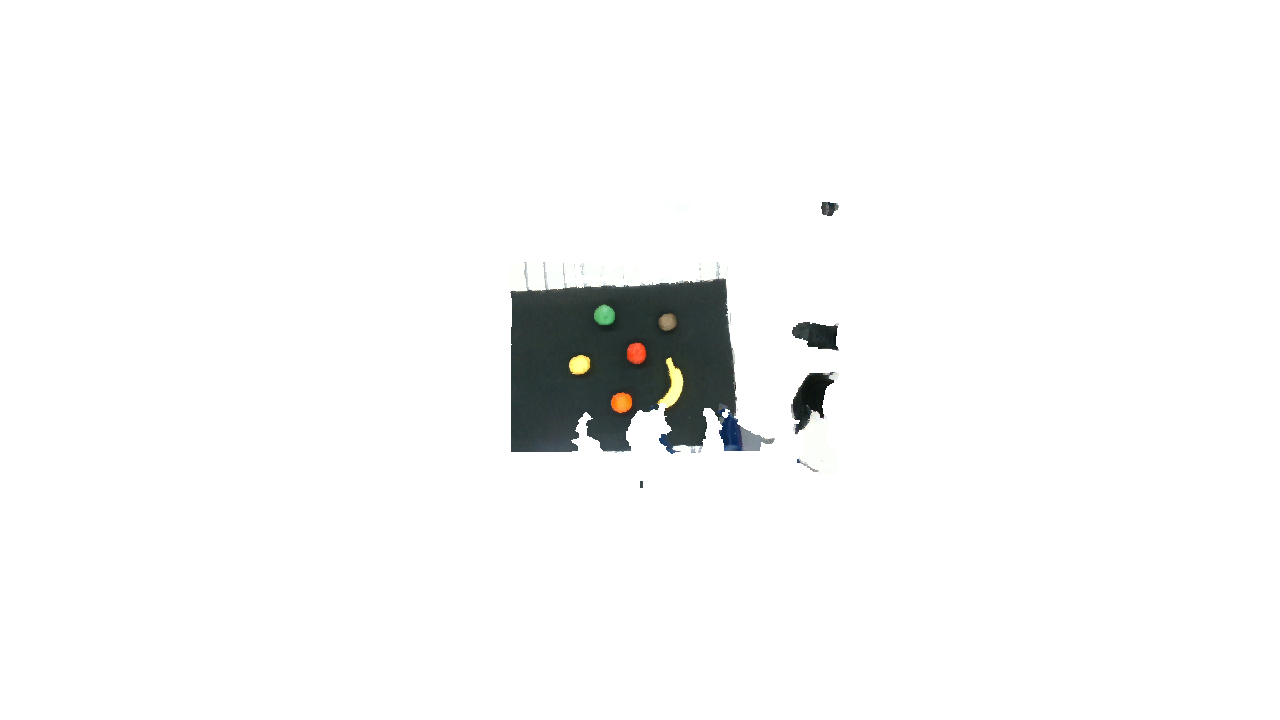
\includegraphics[width=0.48\textwidth]{assets/run_1/step_01_view_1_original.png}
    \hfill
    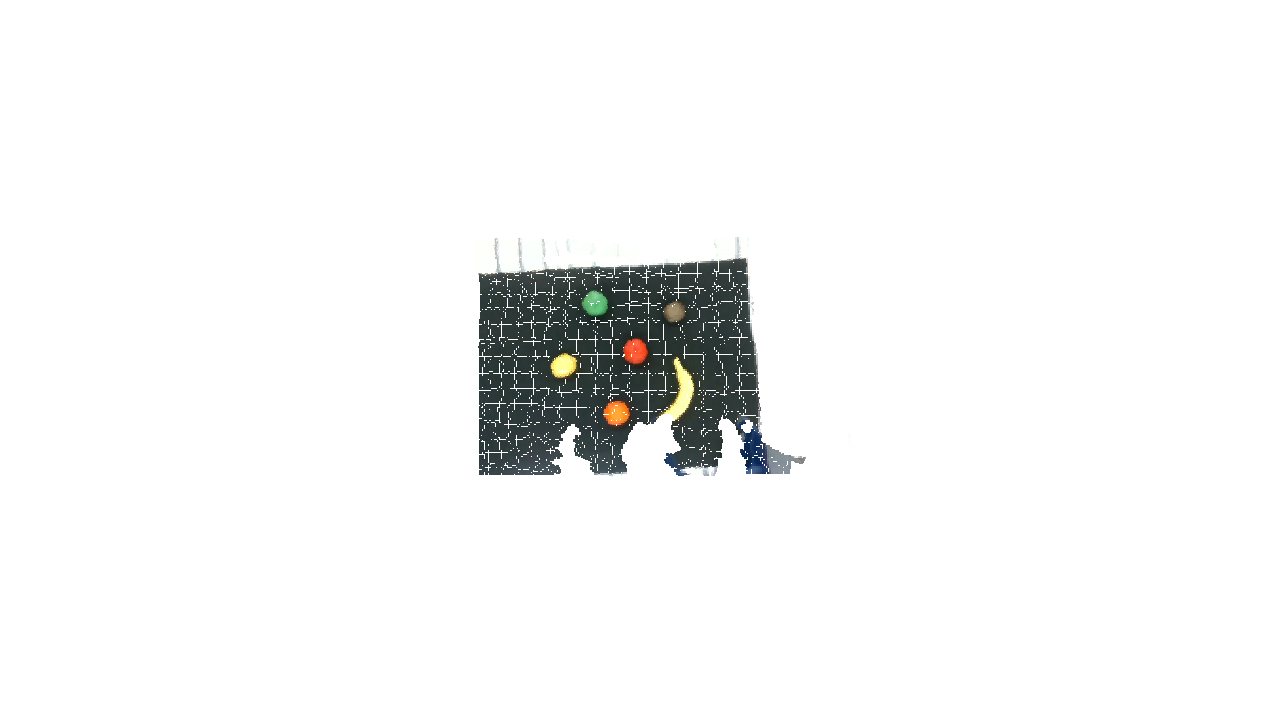
\includegraphics[width=0.48\textwidth]{assets/run_1/step_02_view_1_filtered.png}
    \caption{RUN 1: Originalni oblak točaka (lijevo) i profiltrirani oblak (desno).}
\end{figure}

\begin{figure}[ht]
    \centering
    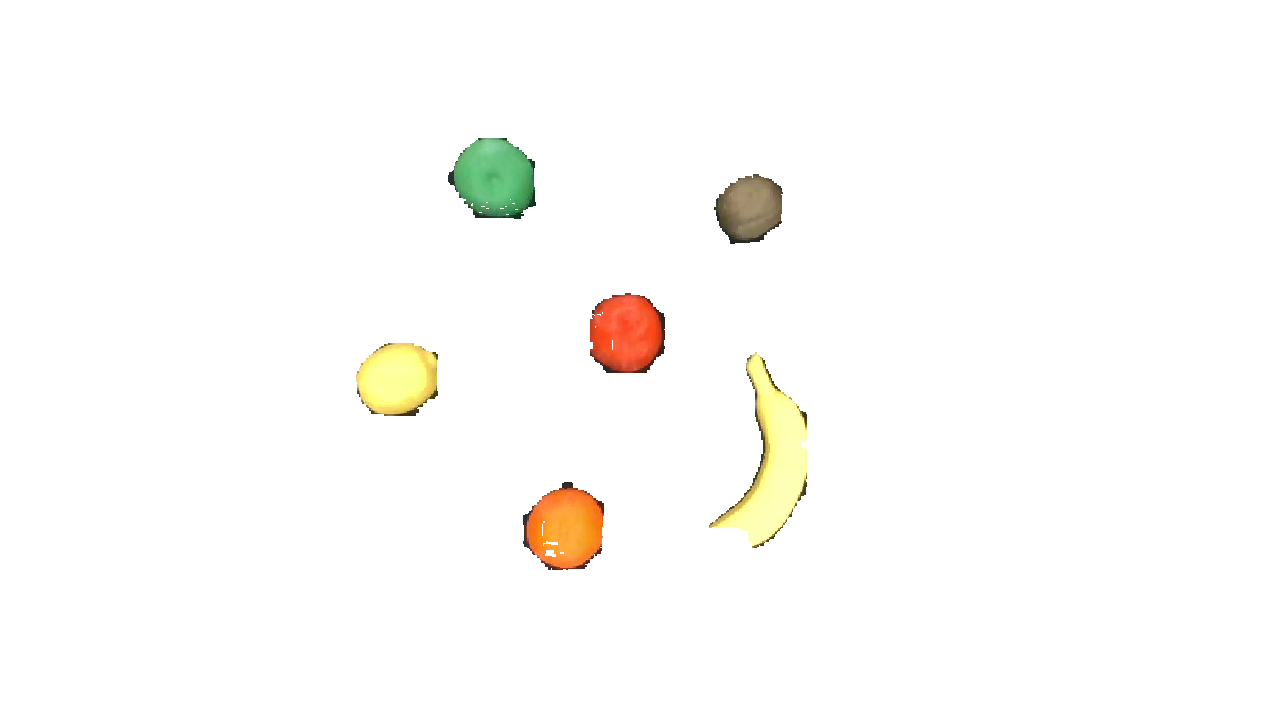
\includegraphics[width=0.48\textwidth]{assets/run_1/step_03_view_1_segmented.png}
    \hfill
    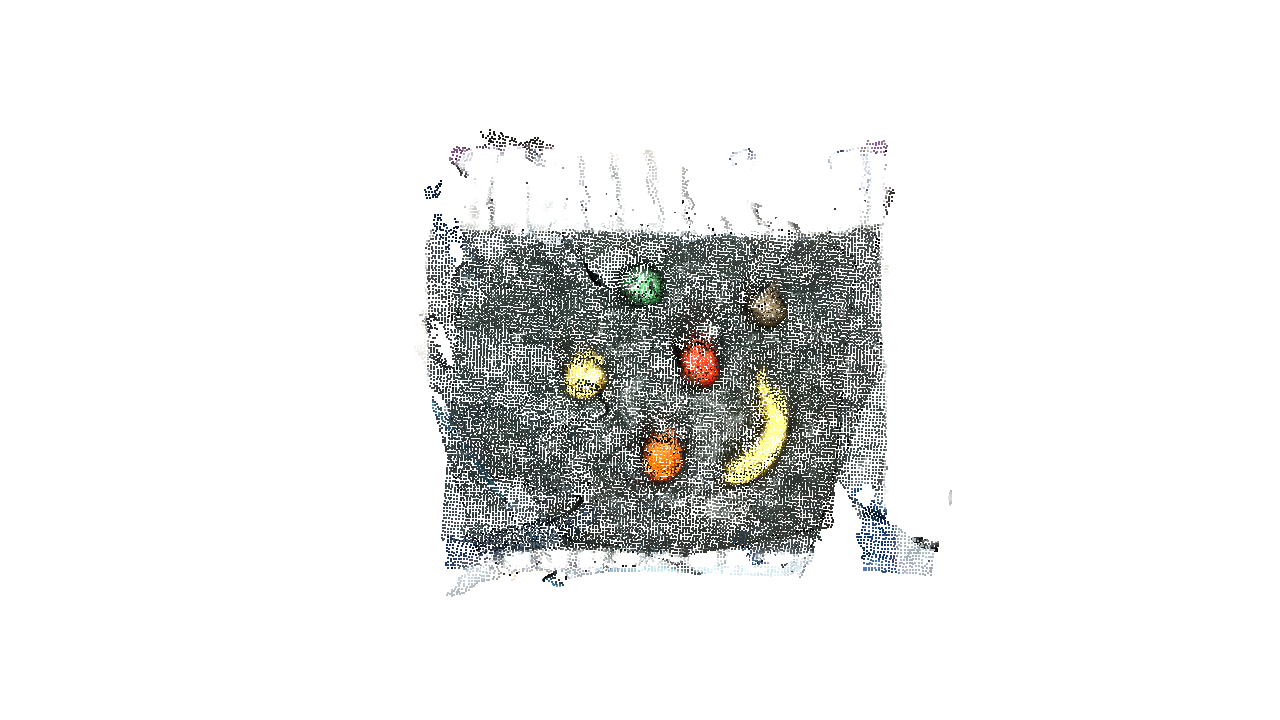
\includegraphics[width=0.48\textwidth]{assets/run_1/step_10_final_merged.png}
    \caption{RUN 1: Segmentirani oblaci za jedan pogled (lijevo) te konačni registrirani globalni oblak nakon ICP-a (desno).}
\end{figure}

\begin{figure}[ht]
    \centering
    
\includegraphics[width=0.48\textwidth]{assets/run_2/step_01_view_1_original.png}
    \hfill
    
\includegraphics[width=0.48\textwidth]{assets/run_2/step_02_view_1_filtered.png}
    \caption{RUN 2: Originalni oblak točaka (lijevo) i profiltrirani oblak (desno).}
\end{figure}

\begin{figure}[ht]
    \centering
    
\includegraphics[width=0.48\textwidth]{assets/run_2/step_03_view_1_segmented.png}
    \hfill
    
\includegraphics[width=0.48\textwidth]{assets/run_2/step_10_final_merged.png}
    \caption{RUN 2: Segmentirani oblaci za jedan pogled (lijevo) te konačni registrirani globalni oblak nakon ICP-a (desno).}
\end{figure}

\section{DETEKCIJA OBJEKATA}
Segmentacija se vrši nad RGB slikom (1280x720) pomoću treniranog YOLO (You Only Look Once) konvolucijskog modela specijaliziranog za maske objekata, uz parametar \texttt{confidence\_threshold = 0.75}. Kroz YOLO detekciju, osim bounding-boxa, dobiva se poligonalna maska. Ta se maska translatira nad dubinsku sliku kako bi se isjekao pripadajući dio Point Clouda.

Da bi se precizno locirao centar voća za zadatak podizanja (\textit{picking}), provodi se postupak:
1. Filtriranje točaka izvan 2D maske.
2. Grupiranje DBSCAN metodom radi odbacivanja krivo klasificiranih rubnih točaka i prljavštine sa stola (najveći klaster proglašava se validnim voćem).
3. Računanje 3D prosjeka koordinata svih preostalih točaka klastera (centroid).
4. Budući da centroid leži blizu geometrijskog središta voća, točka zahvata pomaknuta je u minus smjeru Z osi (iz perspektive TCP-a, tj. gore) za ugrađeni $Z\_offset=-0.02$ m (20 mm) kako hvataljka ne bi udarila o vrh voća.

\begin{figure}[ht]
    \centering
    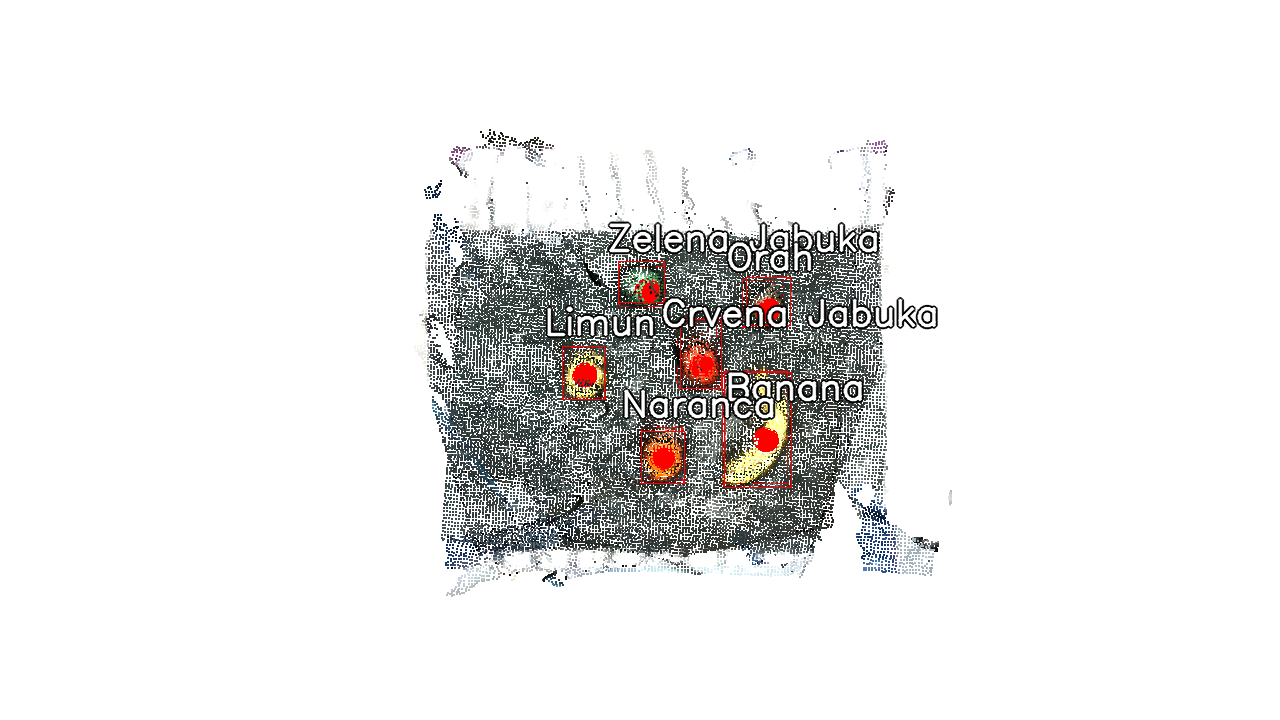
\includegraphics[width=0.48\textwidth]{assets/run_1/step_11_final_classification.png}
    \hfill
    
\includegraphics[width=0.48\textwidth]{assets/run_2/step_11_final_classification.png}
    \caption{Vizualizacija detekcije objekata s pridruženim bounding-box okvirom (lijevo: RUN 1, desno: RUN 2).}
\end{figure}

\section{GENERIRANJE I ANALIZA TRAJEKTORIJE}
Trajektorija kretanja od početne pozicije pa sve do ciljnog kontejnera za odlaganje računa se na razini *task-spacea*. Za interpolaciju između kontrolnih točaka (Home $\to$ Approach $\to$ Pick $\to$ Approach Place $\to$ Place) koristi se \textbf{kvintički polinom} (polinom 5. stupnja), čime se osigurava neprekidnost funkcije puta, brzine te ubrzanja ($C^2$ glatkoća).

Vremena pojedinih faza ($T_1, T_2, \dots$) ovise o euklidskoj udaljenosti i zadanim maksimalnim kinematičkim ograničenjima robota (vmax = $0.25$ m/s, amax = $0.5$ m/s$^2$). Prilikom generiranja trajektorija obavlja se \textbf{diskretizacija} izračunatih funkcija s frekvencijom od 20 Hz, odnosno vremenskim korakom $dt = 0.05$ s. Na ovaj način robot neprekidno prima niz uzastopnih pozicija i brzina te linearno i ravnomjerno komunicira s kontrolerom.

Slika 5 prikazuje grafove pozicije, brzine i ubrzanja u vremenu za prvu međutrajektoriju (od $home0$ do $iznad\_pick1$). Slika 6 donosi vizualizaciju izvedive 3D putanje s istaknutih 5 glavnih TCP poza: $home0$, $iznad\_pick1$, $pick2$, $iznad\_place3$, $place4$. U Tablici 1 prikazana je kvantitativna analiza jedne cjelovite trajektorije s vremenima izvođenja pojedinih međutrajektorija (ukupno 13.0 s). Kako bi se prikazao proces diskretizacije u potpunosti, sve generirane točke unutar ovog ciklusa izlistane su u Dodatku B na kraju dokumenta.

\begin{table}[h]
    \centering
    \caption{Generirane točke i vremena međutrajektorija za ciklus prijenosa voća.}
    \begin{tabular}{|l|c|c|c|c|c|}
        \hline
        \textbf{Poza (Waypoint)} & \textbf{Vrijeme $t$ [s]} & \textbf{$\Delta t$ [s]} & \textbf{$X$ [m]} & \textbf{$Y$ [m]} & \textbf{$Z$ [m]} \\
        \hline
        P1: Home & 0.0 & - & -0.5437 & 0.0935 & 0.1911 \\
        P2: Approach (Pick) & 2.5 & 2.5 & -0.5991 & 0.2271 & 0.1239 \\
        P3: Pick & 4.0 & 1.5 & -0.5991 & 0.2271 & 0.0239 \\
        P4: Retreat (Pick) & 5.5 & 1.5 & -0.5991 & 0.2271 & 0.1239 \\
        P5: Approach (Place) & 8.0 & 2.5 & -0.5466 & 0.2865 & 0.1122 \\
        P6: Place & 9.5 & 1.5 & -0.5466 & 0.2865 & 0.0122 \\
        P7: Retreat (Place) & 11.0 & 1.5 & -0.5466 & 0.2865 & 0.1122 \\
        P8: Home & 13.0 & 2.0 & -0.5437 & 0.0935 & 0.1911 \\
        \hline
    \end{tabular}
\end{table}

\begin{figure}[ht]
    \centering
    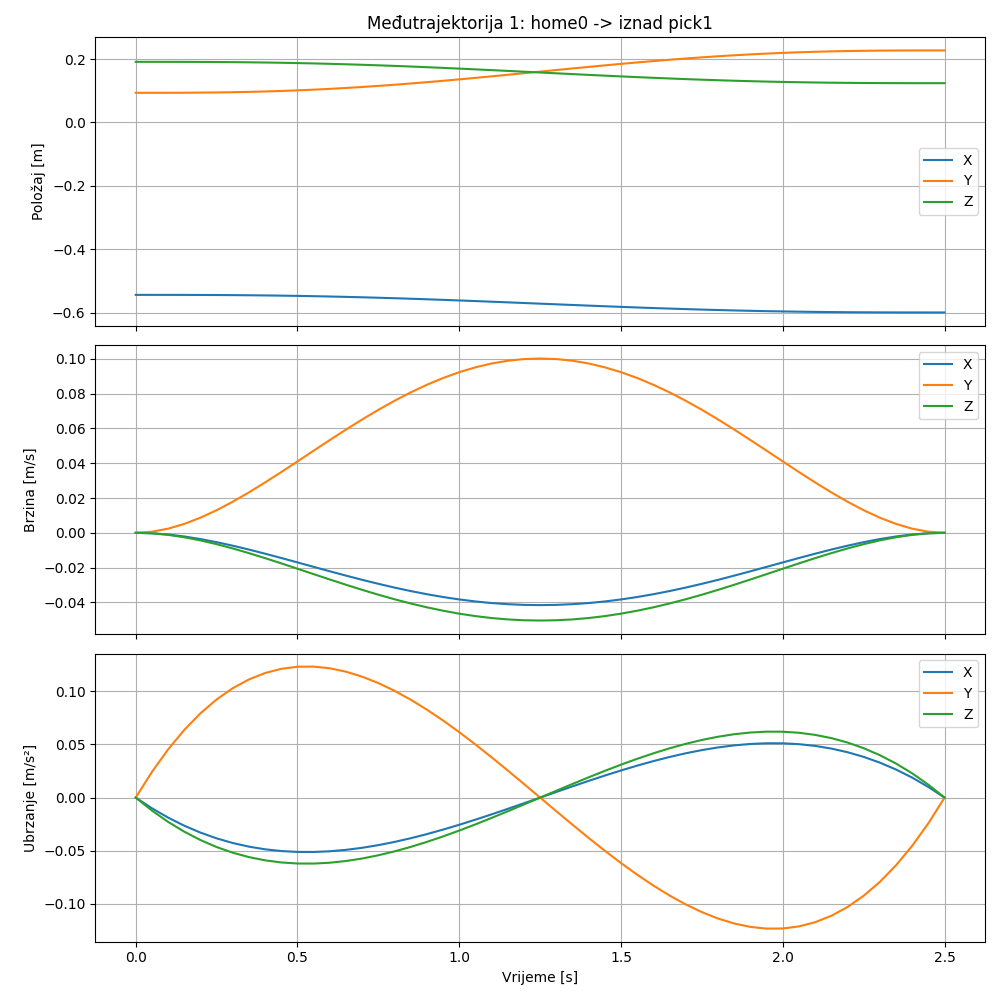
\includegraphics[width=0.75\textwidth]{assets/trajectory_kinematics.png}
    \caption{Kinematička analiza $x_t$, $\dot{x}_t$ i $\ddot{x}_t$ prve međutrajektorije ($home0 \to iznad\_pick1$) - kvintička interpolacija osigurava glatko pokretanje (brzina i ubrzanje na rubovima segmenta jednaki su nuli).}
\end{figure}

\begin{figure}[ht]
    \centering
    
\includegraphics[width=0.75\textwidth]{assets/trajectory_3d_path.png}
    \caption{3D prikaz putanje centralne točke (TCP) sa svih međutrajektorijama i 5 istaknutih TCP poza za zahvat i odlaganje.}
\end{figure}

\newpage
\section*{DODATAK A: GITHUB REPOZITORIJ}
\addcontentsline{toc}{section}{DODATAK A: GITHUB REPOZITORIJ}

Cjelokupni izvorni kod razvijenog rješenja dostupan je na javnom GitHub repozitoriju na sljedećoj poveznici:

\begin{center}
    \url{https://github.com/KxHartl/humanoidna/tree/main/zadaca_03}
\end{center}

\newpage
\section*{DODATAK B: DISKRETIZIRANA TRAJEKTORIJA}
\addcontentsline{toc}{section}{DODATAK B: DISKRETIZIRANA TRAJEKTORIJA}

U tablici u nastavku navedene su koordinate svih 261 izračunatih točaka koje sačinjavaju cjelovitu trajektoriju prikaza u Slici 6, diskretiziranih s vremenskim korakom $dt = 0.05$ s.

\begin{longtable}{|c|c|c|c|c|c|c|}
\caption{Sve generirane točke kompletne izvedbene trajektorije s korakom diskretizacije $dt = 0.05$ s.} \label{tab:all_points} \\
\hline
\textbf{Vrijeme $t$ [s]} & \textbf{$X$ [m]} & \textbf{$Y$ [m]} & \textbf{$Z$ [m]} & \textbf{$R_X$ [rad]} & \textbf{$R_Y$ [rad]} & \textbf{$R_Z$ [rad]} \\
\hline
\endfirsthead

\multicolumn{7}{c}%
{{\bfseries \tablename\ \thetable{} -- nastavak s prethodne stranice}} \\
\hline
\textbf{Vrijeme $t$ [s]} & \textbf{$X$ [m]} & \textbf{$Y$ [m]} & \textbf{$Z$ [m]} & \textbf{$R_X$ [rad]} & \textbf{$R_Y$ [rad]} & \textbf{$R_Z$ [rad]} \\
\hline
\endhead

\hline \multicolumn{7}{|r|}{{Nastavak na sljedećoj stranici...}} \\
\hline
\endfoot

\hline
\endlastfoot

0.00 & -0.5437 & 0.0935 & 0.1911 & 0.0400 & 3.1460 & -0.0510 \\
0.05 & -0.5437 & 0.0935 & 0.1911 & 0.0400 & 3.1460 & -0.0510 \\
0.10 & -0.5437 & 0.0936 & 0.1911 & 0.0400 & 3.1460 & -0.0510 \\
0.15 & -0.5438 & 0.0938 & 0.1910 & 0.0400 & 3.1460 & -0.0510 \\
0.20 & -0.5439 & 0.0941 & 0.1908 & 0.0400 & 3.1460 & -0.0510 \\
0.25 & -0.5441 & 0.0946 & 0.1906 & 0.0400 & 3.1460 & -0.0510 \\
0.30 & -0.5445 & 0.0954 & 0.1902 & 0.0400 & 3.1460 & -0.0510 \\
0.35 & -0.5449 & 0.0964 & 0.1897 & 0.0400 & 3.1460 & -0.0510 \\
0.40 & -0.5454 & 0.0977 & 0.1890 & 0.0400 & 3.1460 & -0.0510 \\
0.45 & -0.5461 & 0.0993 & 0.1882 & 0.0400 & 3.1460 & -0.0510 \\
0.50 & -0.5469 & 0.1012 & 0.1873 & 0.0400 & 3.1460 & -0.0510 \\
0.55 & -0.5478 & 0.1034 & 0.1861 & 0.0400 & 3.1460 & -0.0510 \\
0.60 & -0.5488 & 0.1060 & 0.1849 & 0.0400 & 3.1460 & -0.0510 \\
0.65 & -0.5500 & 0.1088 & 0.1835 & 0.0400 & 3.1460 & -0.0510 \\
0.70 & -0.5513 & 0.1119 & 0.1819 & 0.0400 & 3.1460 & -0.0510 \\
0.75 & -0.5527 & 0.1153 & 0.1802 & 0.0400 & 3.1460 & -0.0510 \\
0.80 & -0.5542 & 0.1190 & 0.1783 & 0.0400 & 3.1460 & -0.0510 \\
0.85 & -0.5558 & 0.1229 & 0.1764 & 0.0400 & 3.1460 & -0.0510 \\
0.90 & -0.5576 & 0.1270 & 0.1743 & 0.0400 & 3.1460 & -0.0510 \\
0.95 & -0.5594 & 0.1314 & 0.1721 & 0.0400 & 3.1460 & -0.0510 \\
1.00 & -0.5613 & 0.1359 & 0.1698 & 0.0400 & 3.1460 & -0.0510 \\
1.05 & -0.5632 & 0.1406 & 0.1674 & 0.0400 & 3.1460 & -0.0510 \\
1.10 & -0.5652 & 0.1454 & 0.1650 & 0.0400 & 3.1460 & -0.0510 \\
1.15 & -0.5672 & 0.1503 & 0.1625 & 0.0400 & 3.1460 & -0.0510 \\
1.20 & -0.5693 & 0.1553 & 0.1600 & 0.0400 & 3.1460 & -0.0510 \\
1.25 & -0.5714 & 0.1603 & 0.1575 & 0.0400 & 3.1460 & -0.0510 \\
1.30 & -0.5735 & 0.1653 & 0.1550 & 0.0400 & 3.1460 & -0.0510 \\
1.35 & -0.5755 & 0.1703 & 0.1525 & 0.0400 & 3.1460 & -0.0510 \\
1.40 & -0.5776 & 0.1752 & 0.1500 & 0.0400 & 3.1460 & -0.0510 \\
1.45 & -0.5796 & 0.1800 & 0.1476 & 0.0400 & 3.1460 & -0.0510 \\
1.50 & -0.5815 & 0.1847 & 0.1452 & 0.0400 & 3.1460 & -0.0510 \\
1.55 & -0.5834 & 0.1892 & 0.1430 & 0.0400 & 3.1460 & -0.0510 \\
1.60 & -0.5852 & 0.1936 & 0.1408 & 0.0400 & 3.1460 & -0.0510 \\
1.65 & -0.5869 & 0.1977 & 0.1387 & 0.0400 & 3.1460 & -0.0510 \\
1.70 & -0.5885 & 0.2017 & 0.1367 & 0.0400 & 3.1460 & -0.0510 \\
1.75 & -0.5901 & 0.2053 & 0.1349 & 0.0400 & 3.1460 & -0.0510 \\
1.80 & -0.5915 & 0.2087 & 0.1331 & 0.0400 & 3.1460 & -0.0510 \\
1.85 & -0.5928 & 0.2118 & 0.1316 & 0.0400 & 3.1460 & -0.0510 \\
1.90 & -0.5939 & 0.2147 & 0.1302 & 0.0400 & 3.1460 & -0.0510 \\
1.95 & -0.5950 & 0.2172 & 0.1289 & 0.0400 & 3.1460 & -0.0510 \\
2.00 & -0.5959 & 0.2194 & 0.1278 & 0.0400 & 3.1460 & -0.0510 \\
2.05 & -0.5967 & 0.2213 & 0.1268 & 0.0400 & 3.1460 & -0.0510 \\
2.10 & -0.5973 & 0.2229 & 0.1260 & 0.0400 & 3.1460 & -0.0510 \\
2.15 & -0.5979 & 0.2242 & 0.1254 & 0.0400 & 3.1460 & -0.0510 \\
2.20 & -0.5983 & 0.2252 & 0.1248 & 0.0400 & 3.1460 & -0.0510 \\
2.25 & -0.5986 & 0.2260 & 0.1245 & 0.0400 & 3.1460 & -0.0510 \\
2.30 & -0.5989 & 0.2265 & 0.1242 & 0.0400 & 3.1460 & -0.0510 \\
2.35 & -0.5990 & 0.2268 & 0.1240 & 0.0400 & 3.1460 & -0.0510 \\
2.40 & -0.5991 & 0.2270 & 0.1239 & 0.0400 & 3.1460 & -0.0510 \\
2.45 & -0.5991 & 0.2271 & 0.1239 & 0.0400 & 3.1460 & -0.0510 \\
2.50 & -0.5991 & 0.2271 & 0.1239 & 0.0400 & 3.1460 & -0.0510 \\
2.55 & -0.5991 & 0.2271 & 0.1238 & 0.0400 & 3.1460 & -0.0510 \\
2.60 & -0.5991 & 0.2271 & 0.1236 & 0.0400 & 3.1460 & -0.0510 \\
2.65 & -0.5991 & 0.2271 & 0.1230 & 0.0400 & 3.1460 & -0.0510 \\
2.70 & -0.5991 & 0.2271 & 0.1220 & 0.0400 & 3.1460 & -0.0510 \\
2.75 & -0.5991 & 0.2271 & 0.1203 & 0.0400 & 3.1460 & -0.0510 \\
2.80 & -0.5991 & 0.2271 & 0.1181 & 0.0400 & 3.1460 & -0.0510 \\
2.85 & -0.5991 & 0.2271 & 0.1152 & 0.0400 & 3.1460 & -0.0510 \\
2.90 & -0.5991 & 0.2271 & 0.1117 & 0.0400 & 3.1460 & -0.0510 \\
2.95 & -0.5991 & 0.2271 & 0.1076 & 0.0400 & 3.1460 & -0.0510 \\
3.00 & -0.5991 & 0.2271 & 0.1029 & 0.0400 & 3.1460 & -0.0510 \\
3.05 & -0.5991 & 0.2271 & 0.0977 & 0.0400 & 3.1460 & -0.0510 \\
3.10 & -0.5991 & 0.2271 & 0.0921 & 0.0400 & 3.1460 & -0.0510 \\
3.15 & -0.5991 & 0.2271 & 0.0862 & 0.0400 & 3.1460 & -0.0510 \\
3.20 & -0.5991 & 0.2271 & 0.0801 & 0.0400 & 3.1460 & -0.0510 \\
3.25 & -0.5991 & 0.2271 & 0.0739 & 0.0400 & 3.1460 & -0.0510 \\
3.30 & -0.5991 & 0.2271 & 0.0676 & 0.0400 & 3.1460 & -0.0510 \\
3.35 & -0.5991 & 0.2271 & 0.0615 & 0.0400 & 3.1460 & -0.0510 \\
3.40 & -0.5991 & 0.2271 & 0.0556 & 0.0400 & 3.1460 & -0.0510 \\
3.45 & -0.5991 & 0.2271 & 0.0500 & 0.0400 & 3.1460 & -0.0510 \\
3.50 & -0.5991 & 0.2271 & 0.0449 & 0.0400 & 3.1460 & -0.0510 \\
3.55 & -0.5991 & 0.2271 & 0.0402 & 0.0400 & 3.1460 & -0.0510 \\
3.60 & -0.5991 & 0.2271 & 0.0361 & 0.0400 & 3.1460 & -0.0510 \\
3.65 & -0.5991 & 0.2271 & 0.0326 & 0.0400 & 3.1460 & -0.0510 \\
3.70 & -0.5991 & 0.2271 & 0.0297 & 0.0400 & 3.1460 & -0.0510 \\
3.75 & -0.5991 & 0.2271 & 0.0274 & 0.0400 & 3.1460 & -0.0510 \\
3.80 & -0.5991 & 0.2271 & 0.0258 & 0.0400 & 3.1460 & -0.0510 \\
3.85 & -0.5991 & 0.2271 & 0.0247 & 0.0400 & 3.1460 & -0.0510 \\
3.90 & -0.5991 & 0.2271 & 0.0241 & 0.0400 & 3.1460 & -0.0510 \\
3.95 & -0.5991 & 0.2271 & 0.0239 & 0.0400 & 3.1460 & -0.0510 \\
4.00 & -0.5991 & 0.2271 & 0.0239 & 0.0400 & 3.1460 & -0.0510 \\
4.05 & -0.5991 & 0.2271 & 0.0239 & 0.0400 & 3.1460 & -0.0510 \\
4.10 & -0.5991 & 0.2271 & 0.0241 & 0.0400 & 3.1460 & -0.0510 \\
4.15 & -0.5991 & 0.2271 & 0.0247 & 0.0400 & 3.1460 & -0.0510 \\
4.20 & -0.5991 & 0.2271 & 0.0258 & 0.0400 & 3.1460 & -0.0510 \\
4.25 & -0.5991 & 0.2271 & 0.0274 & 0.0400 & 3.1460 & -0.0510 \\
4.30 & -0.5991 & 0.2271 & 0.0297 & 0.0400 & 3.1460 & -0.0510 \\
4.35 & -0.5991 & 0.2271 & 0.0326 & 0.0400 & 3.1460 & -0.0510 \\
4.40 & -0.5991 & 0.2271 & 0.0361 & 0.0400 & 3.1460 & -0.0510 \\
4.45 & -0.5991 & 0.2271 & 0.0402 & 0.0400 & 3.1460 & -0.0510 \\
4.50 & -0.5991 & 0.2271 & 0.0449 & 0.0400 & 3.1460 & -0.0510 \\
4.55 & -0.5991 & 0.2271 & 0.0500 & 0.0400 & 3.1460 & -0.0510 \\
4.60 & -0.5991 & 0.2271 & 0.0556 & 0.0400 & 3.1460 & -0.0510 \\
4.65 & -0.5991 & 0.2271 & 0.0615 & 0.0400 & 3.1460 & -0.0510 \\
4.70 & -0.5991 & 0.2271 & 0.0676 & 0.0400 & 3.1460 & -0.0510 \\
4.75 & -0.5991 & 0.2271 & 0.0739 & 0.0400 & 3.1460 & -0.0510 \\
4.80 & -0.5991 & 0.2271 & 0.0801 & 0.0400 & 3.1460 & -0.0510 \\
4.85 & -0.5991 & 0.2271 & 0.0862 & 0.0400 & 3.1460 & -0.0510 \\
4.90 & -0.5991 & 0.2271 & 0.0921 & 0.0400 & 3.1460 & -0.0510 \\
4.95 & -0.5991 & 0.2271 & 0.0977 & 0.0400 & 3.1460 & -0.0510 \\
5.00 & -0.5991 & 0.2271 & 0.1029 & 0.0400 & 3.1460 & -0.0510 \\
5.05 & -0.5991 & 0.2271 & 0.1076 & 0.0400 & 3.1460 & -0.0510 \\
5.10 & -0.5991 & 0.2271 & 0.1117 & 0.0400 & 3.1460 & -0.0510 \\
5.15 & -0.5991 & 0.2271 & 0.1152 & 0.0400 & 3.1460 & -0.0510 \\
5.20 & -0.5991 & 0.2271 & 0.1181 & 0.0400 & 3.1460 & -0.0510 \\
5.25 & -0.5991 & 0.2271 & 0.1203 & 0.0400 & 3.1460 & -0.0510 \\
5.30 & -0.5991 & 0.2271 & 0.1220 & 0.0400 & 3.1460 & -0.0510 \\
5.35 & -0.5991 & 0.2271 & 0.1230 & 0.0400 & 3.1460 & -0.0510 \\
5.40 & -0.5991 & 0.2271 & 0.1236 & 0.0400 & 3.1460 & -0.0510 \\
5.45 & -0.5991 & 0.2271 & 0.1238 & 0.0400 & 3.1460 & -0.0510 \\
5.50 & -0.5991 & 0.2271 & 0.1239 & 0.0400 & 3.1460 & -0.0510 \\
5.55 & -0.5991 & 0.2271 & 0.1239 & 0.0400 & 3.1460 & -0.0510 \\
5.60 & -0.5991 & 0.2271 & 0.1239 & 0.0403 & 3.1460 & -0.0509 \\
5.65 & -0.5990 & 0.2272 & 0.1239 & 0.0409 & 3.1459 & -0.0508 \\
5.70 & -0.5989 & 0.2274 & 0.1238 & 0.0421 & 3.1458 & -0.0505 \\
5.75 & -0.5987 & 0.2276 & 0.1238 & 0.0440 & 3.1457 & -0.0501 \\
5.80 & -0.5984 & 0.2280 & 0.1237 & 0.0468 & 3.1455 & -0.0494 \\
5.85 & -0.5979 & 0.2284 & 0.1236 & 0.0504 & 3.1452 & -0.0486 \\
5.90 & -0.5974 & 0.2290 & 0.1235 & 0.0550 & 3.1449 & -0.0475 \\
5.95 & -0.5968 & 0.2297 & 0.1234 & 0.0606 & 3.1445 & -0.0462 \\
6.00 & -0.5961 & 0.2305 & 0.1232 & 0.0673 & 3.1440 & -0.0446 \\
6.05 & -0.5952 & 0.2315 & 0.1230 & 0.0751 & 3.1434 & -0.0428 \\
6.10 & -0.5942 & 0.2326 & 0.1228 & 0.0840 & 3.1427 & -0.0407 \\
6.15 & -0.5931 & 0.2339 & 0.1225 & 0.0940 & 3.1420 & -0.0384 \\
6.20 & -0.5919 & 0.2353 & 0.1223 & 0.1050 & 3.1412 & -0.0359 \\
6.25 & -0.5905 & 0.2368 & 0.1220 & 0.1170 & 3.1403 & -0.0331 \\
6.30 & -0.5891 & 0.2384 & 0.1217 & 0.1299 & 3.1393 & -0.0300 \\
6.35 & -0.5876 & 0.2402 & 0.1213 & 0.1438 & 3.1383 & -0.0268 \\
6.40 & -0.5859 & 0.2420 & 0.1209 & 0.1584 & 3.1372 & -0.0234 \\
6.45 & -0.5842 & 0.2439 & 0.1206 & 0.1738 & 3.1361 & -0.0198 \\
6.50 & -0.5824 & 0.2460 & 0.1202 & 0.1898 & 3.1349 & -0.0161 \\
6.55 & -0.5806 & 0.2480 & 0.1198 & 0.2064 & 3.1337 & -0.0122 \\
6.60 & -0.5787 & 0.2502 & 0.1193 & 0.2234 & 3.1324 & -0.0083 \\
6.65 & -0.5768 & 0.2524 & 0.1189 & 0.2408 & 3.1311 & -0.0042 \\
6.70 & -0.5748 & 0.2546 & 0.1185 & 0.2583 & 3.1298 & -0.0001 \\
6.75 & -0.5729 & 0.2568 & 0.1180 & 0.2760 & 3.1285 & 0.0040 \\
6.80 & -0.5709 & 0.2590 & 0.1176 & 0.2937 & 3.1272 & 0.0081 \\
6.85 & -0.5689 & 0.2612 & 0.1172 & 0.3112 & 3.1259 & 0.0122 \\
6.90 & -0.5670 & 0.2634 & 0.1167 & 0.3286 & 3.1246 & 0.0163 \\
6.95 & -0.5651 & 0.2655 & 0.1163 & 0.3456 & 3.1233 & 0.0202 \\
7.00 & -0.5633 & 0.2676 & 0.1159 & 0.3622 & 3.1221 & 0.0241 \\
7.05 & -0.5615 & 0.2696 & 0.1155 & 0.3782 & 3.1209 & 0.0278 \\
7.10 & -0.5598 & 0.2716 & 0.1151 & 0.3936 & 3.1198 & 0.0314 \\
7.15 & -0.5582 & 0.2734 & 0.1148 & 0.4082 & 3.1187 & 0.0348 \\
7.20 & -0.5566 & 0.2752 & 0.1144 & 0.4221 & 3.1177 & 0.0380 \\
7.25 & -0.5552 & 0.2768 & 0.1141 & 0.4350 & 3.1167 & 0.0411 \\
7.30 & -0.5538 & 0.2783 & 0.1138 & 0.4470 & 3.1158 & 0.0439 \\
7.35 & -0.5526 & 0.2797 & 0.1135 & 0.4580 & 3.1150 & 0.0464 \\
7.40 & -0.5515 & 0.2809 & 0.1133 & 0.4680 & 3.1143 & 0.0487 \\
7.45 & -0.5505 & 0.2820 & 0.1131 & 0.4769 & 3.1136 & 0.0508 \\
7.50 & -0.5497 & 0.2830 & 0.1129 & 0.4847 & 3.1130 & 0.0526 \\
7.55 & -0.5489 & 0.2839 & 0.1127 & 0.4914 & 3.1125 & 0.0542 \\
7.60 & -0.5483 & 0.2846 & 0.1126 & 0.4970 & 3.1121 & 0.0555 \\
7.65 & -0.5478 & 0.2852 & 0.1124 & 0.5016 & 3.1118 & 0.0566 \\
7.70 & -0.5474 & 0.2856 & 0.1123 & 0.5052 & 3.1115 & 0.0574 \\
7.75 & -0.5471 & 0.2860 & 0.1123 & 0.5080 & 3.1113 & 0.0581 \\
7.80 & -0.5468 & 0.2862 & 0.1122 & 0.5099 & 3.1112 & 0.0585 \\
7.85 & -0.5467 & 0.2863 & 0.1122 & 0.5111 & 3.1111 & 0.0588 \\
7.90 & -0.5466 & 0.2864 & 0.1122 & 0.5117 & 3.1110 & 0.0589 \\
7.95 & -0.5466 & 0.2865 & 0.1122 & 0.5120 & 3.1110 & 0.0590 \\
8.00 & -0.5466 & 0.2865 & 0.1122 & 0.5120 & 3.1110 & 0.0590 \\
8.05 & -0.5466 & 0.2865 & 0.1121 & 0.5120 & 3.1110 & 0.0590 \\
8.10 & -0.5466 & 0.2865 & 0.1119 & 0.5120 & 3.1110 & 0.0590 \\
8.15 & -0.5466 & 0.2865 & 0.1113 & 0.5120 & 3.1110 & 0.0590 \\
8.20 & -0.5466 & 0.2865 & 0.1103 & 0.5120 & 3.1110 & 0.0590 \\
8.25 & -0.5466 & 0.2865 & 0.1086 & 0.5120 & 3.1110 & 0.0590 \\
8.30 & -0.5466 & 0.2865 & 0.1064 & 0.5120 & 3.1110 & 0.0590 \\
8.35 & -0.5466 & 0.2865 & 0.1035 & 0.5120 & 3.1110 & 0.0590 \\
8.40 & -0.5466 & 0.2865 & 0.1000 & 0.5120 & 3.1110 & 0.0590 \\
8.45 & -0.5466 & 0.2865 & 0.0959 & 0.5120 & 3.1110 & 0.0590 \\
8.50 & -0.5466 & 0.2865 & 0.0912 & 0.5120 & 3.1110 & 0.0590 \\
8.55 & -0.5466 & 0.2865 & 0.0860 & 0.5120 & 3.1110 & 0.0590 \\
8.60 & -0.5466 & 0.2865 & 0.0804 & 0.5120 & 3.1110 & 0.0590 \\
8.65 & -0.5466 & 0.2865 & 0.0745 & 0.5120 & 3.1110 & 0.0590 \\
8.70 & -0.5466 & 0.2865 & 0.0684 & 0.5120 & 3.1110 & 0.0590 \\
8.75 & -0.5466 & 0.2865 & 0.0622 & 0.5120 & 3.1110 & 0.0590 \\
8.80 & -0.5466 & 0.2865 & 0.0559 & 0.5120 & 3.1110 & 0.0590 \\
8.85 & -0.5466 & 0.2865 & 0.0498 & 0.5120 & 3.1110 & 0.0590 \\
8.90 & -0.5466 & 0.2865 & 0.0439 & 0.5120 & 3.1110 & 0.0590 \\
8.95 & -0.5466 & 0.2865 & 0.0383 & 0.5120 & 3.1110 & 0.0590 \\
9.00 & -0.5466 & 0.2865 & 0.0332 & 0.5120 & 3.1110 & 0.0590 \\
9.05 & -0.5466 & 0.2865 & 0.0285 & 0.5120 & 3.1110 & 0.0590 \\
9.10 & -0.5466 & 0.2865 & 0.0244 & 0.5120 & 3.1110 & 0.0590 \\
9.15 & -0.5466 & 0.2865 & 0.0209 & 0.5120 & 3.1110 & 0.0590 \\
9.20 & -0.5466 & 0.2865 & 0.0180 & 0.5120 & 3.1110 & 0.0590 \\
9.25 & -0.5466 & 0.2865 & 0.0157 & 0.5120 & 3.1110 & 0.0590 \\
9.30 & -0.5466 & 0.2865 & 0.0141 & 0.5120 & 3.1110 & 0.0590 \\
9.35 & -0.5466 & 0.2865 & 0.0130 & 0.5120 & 3.1110 & 0.0590 \\
9.40 & -0.5466 & 0.2865 & 0.0124 & 0.5120 & 3.1110 & 0.0590 \\
9.45 & -0.5466 & 0.2865 & 0.0122 & 0.5120 & 3.1110 & 0.0590 \\
9.50 & -0.5466 & 0.2865 & 0.0122 & 0.5120 & 3.1110 & 0.0590 \\
9.55 & -0.5466 & 0.2865 & 0.0122 & 0.5120 & 3.1110 & 0.0590 \\
9.60 & -0.5466 & 0.2865 & 0.0124 & 0.5120 & 3.1110 & 0.0590 \\
9.65 & -0.5466 & 0.2865 & 0.0130 & 0.5120 & 3.1110 & 0.0590 \\
9.70 & -0.5466 & 0.2865 & 0.0141 & 0.5120 & 3.1110 & 0.0590 \\
9.75 & -0.5466 & 0.2865 & 0.0157 & 0.5120 & 3.1110 & 0.0590 \\
9.80 & -0.5466 & 0.2865 & 0.0180 & 0.5120 & 3.1110 & 0.0590 \\
9.85 & -0.5466 & 0.2865 & 0.0209 & 0.5120 & 3.1110 & 0.0590 \\
9.90 & -0.5466 & 0.2865 & 0.0244 & 0.5120 & 3.1110 & 0.0590 \\
9.95 & -0.5466 & 0.2865 & 0.0285 & 0.5120 & 3.1110 & 0.0590 \\
10.00 & -0.5466 & 0.2865 & 0.0332 & 0.5120 & 3.1110 & 0.0590 \\
10.05 & -0.5466 & 0.2865 & 0.0383 & 0.5120 & 3.1110 & 0.0590 \\
10.10 & -0.5466 & 0.2865 & 0.0439 & 0.5120 & 3.1110 & 0.0590 \\
10.15 & -0.5466 & 0.2865 & 0.0498 & 0.5120 & 3.1110 & 0.0590 \\
10.20 & -0.5466 & 0.2865 & 0.0559 & 0.5120 & 3.1110 & 0.0590 \\
10.25 & -0.5466 & 0.2865 & 0.0622 & 0.5120 & 3.1110 & 0.0590 \\
10.30 & -0.5466 & 0.2865 & 0.0684 & 0.5120 & 3.1110 & 0.0590 \\
10.35 & -0.5466 & 0.2865 & 0.0745 & 0.5120 & 3.1110 & 0.0590 \\
10.40 & -0.5466 & 0.2865 & 0.0804 & 0.5120 & 3.1110 & 0.0590 \\
10.45 & -0.5466 & 0.2865 & 0.0860 & 0.5120 & 3.1110 & 0.0590 \\
10.50 & -0.5466 & 0.2865 & 0.0912 & 0.5120 & 3.1110 & 0.0590 \\
10.55 & -0.5466 & 0.2865 & 0.0959 & 0.5120 & 3.1110 & 0.0590 \\
10.60 & -0.5466 & 0.2865 & 0.1000 & 0.5120 & 3.1110 & 0.0590 \\
10.65 & -0.5466 & 0.2865 & 0.1035 & 0.5120 & 3.1110 & 0.0590 \\
10.70 & -0.5466 & 0.2865 & 0.1064 & 0.5120 & 3.1110 & 0.0590 \\
10.75 & -0.5466 & 0.2865 & 0.1086 & 0.5120 & 3.1110 & 0.0590 \\
10.80 & -0.5466 & 0.2865 & 0.1103 & 0.5120 & 3.1110 & 0.0590 \\
10.85 & -0.5466 & 0.2865 & 0.1113 & 0.5120 & 3.1110 & 0.0590 \\
10.90 & -0.5466 & 0.2865 & 0.1119 & 0.5120 & 3.1110 & 0.0590 \\
10.95 & -0.5466 & 0.2865 & 0.1121 & 0.5120 & 3.1110 & 0.0590 \\
11.00 & -0.5466 & 0.2865 & 0.1122 & 0.5120 & 3.1110 & 0.0590 \\
11.05 & -0.5466 & 0.2864 & 0.1122 & 0.5119 & 3.1110 & 0.0590 \\
11.10 & -0.5466 & 0.2862 & 0.1123 & 0.5115 & 3.1110 & 0.0589 \\
11.15 & -0.5466 & 0.2857 & 0.1125 & 0.5102 & 3.1111 & 0.0586 \\
11.20 & -0.5466 & 0.2848 & 0.1129 & 0.5080 & 3.1113 & 0.0581 \\
11.25 & -0.5466 & 0.2834 & 0.1134 & 0.5044 & 3.1116 & 0.0572 \\
11.30 & -0.5465 & 0.2813 & 0.1143 & 0.4994 & 3.1119 & 0.0561 \\
11.35 & -0.5465 & 0.2786 & 0.1154 & 0.4929 & 3.1124 & 0.0545 \\
11.40 & -0.5464 & 0.2753 & 0.1168 & 0.4847 & 3.1130 & 0.0526 \\
11.45 & -0.5464 & 0.2712 & 0.1184 & 0.4747 & 3.1138 & 0.0503 \\
11.50 & -0.5463 & 0.2665 & 0.1204 & 0.4631 & 3.1146 & 0.0476 \\
11.55 & -0.5462 & 0.2611 & 0.1226 & 0.4499 & 3.1156 & 0.0445 \\
11.60 & -0.5461 & 0.2550 & 0.1251 & 0.4350 & 3.1167 & 0.0411 \\
11.65 & -0.5460 & 0.2483 & 0.1278 & 0.4187 & 3.1179 & 0.0373 \\
11.70 & -0.5459 & 0.2411 & 0.1308 & 0.4010 & 3.1192 & 0.0331 \\
11.75 & -0.5458 & 0.2334 & 0.1339 & 0.3821 & 3.1206 & 0.0287 \\
11.80 & -0.5457 & 0.2252 & 0.1372 & 0.3622 & 3.1221 & 0.0241 \\
11.85 & -0.5455 & 0.2167 & 0.1407 & 0.3414 & 3.1237 & 0.0192 \\
11.90 & -0.5454 & 0.2079 & 0.1443 & 0.3200 & 3.1252 & 0.0142 \\
11.95 & -0.5453 & 0.1990 & 0.1480 & 0.2981 & 3.1269 & 0.0091 \\
12.00 & -0.5451 & 0.1900 & 0.1517 & 0.2760 & 3.1285 & 0.0040 \\
12.05 & -0.5450 & 0.1810 & 0.1554 & 0.2539 & 3.1301 & -0.0011 \\
12.10 & -0.5449 & 0.1720 & 0.1590 & 0.2320 & 3.1318 & -0.0062 \\
12.15 & -0.5447 & 0.1632 & 0.1626 & 0.2106 & 3.1333 & -0.0112 \\
12.20 & -0.5446 & 0.1548 & 0.1661 & 0.1898 & 3.1349 & -0.0161 \\
12.25 & -0.5445 & 0.1466 & 0.1694 & 0.1699 & 3.1364 & -0.0207 \\
12.30 & -0.5444 & 0.1389 & 0.1726 & 0.1510 & 3.1378 & -0.0251 \\
12.35 & -0.5442 & 0.1316 & 0.1755 & 0.1333 & 3.1391 & -0.0293 \\
12.40 & -0.5441 & 0.1250 & 0.1783 & 0.1170 & 3.1403 & -0.0331 \\
12.45 & -0.5440 & 0.1189 & 0.1808 & 0.1021 & 3.1414 & -0.0365 \\
12.50 & -0.5440 & 0.1135 & 0.1830 & 0.0889 & 3.1424 & -0.0396 \\
12.55 & -0.5439 & 0.1087 & 0.1849 & 0.0773 & 3.1432 & -0.0423 \\
12.60 & -0.5438 & 0.1047 & 0.1866 & 0.0673 & 3.1440 & -0.0446 \\
12.65 & -0.5438 & 0.1013 & 0.1880 & 0.0591 & 3.1446 & -0.0465 \\
12.70 & -0.5437 & 0.0986 & 0.1890 & 0.0526 & 3.1451 & -0.0481 \\
12.75 & -0.5437 & 0.0966 & 0.1899 & 0.0476 & 3.1454 & -0.0492 \\
12.80 & -0.5437 & 0.0952 & 0.1905 & 0.0440 & 3.1457 & -0.0501 \\
12.85 & -0.5437 & 0.0942 & 0.1909 & 0.0418 & 3.1459 & -0.0506 \\
12.90 & -0.5437 & 0.0937 & 0.1911 & 0.0405 & 3.1460 & -0.0509 \\
12.95 & -0.5437 & 0.0935 & 0.1911 & 0.0401 & 3.1460 & -0.0510 \\
13.00 & -0.5437 & 0.0935 & 0.1911 & 0.0400 & 3.1460 & -0.0510 \\
\end{longtable}


\end{document}
